\section*{BT ÔN TẬP KTTX1}
\setcounter{ex}{0}\setcounter{bt}{0}
\Opensolutionfile{ans}[ans/ans1C3-CD-1]
\TN

\begin{ex}%[Tex hóa SGK CD-CT,T12/22, TVN-006]%[1K1Y1-8]
	Trong các khẳng định sau, khẳng định  nào là \textbf{sai}?
	\choice
	{$\sin(\pi-\alpha)=\sin\alpha$}
	{\True $\cos(\pi-\alpha)=\cos \alpha$}
	{$\sin(\pi+\alpha)=-\sin\alpha$}
	{$\cos(\pi+\alpha)=-\cos \alpha$}
	\loigiai{
		Ta có $\cos(\pi-\alpha)=-\cos \alpha$ nên $\cos(\pi-\alpha)=\cos \alpha$ là khẳng định \textbf{sai}.
	}
\end{ex}

\begin{ex}%[1C1B1-2]
	Cho góc lượng giác gốc $O$ có tia đầu $Ou$, tia cuối $Ov$ và có số đo $\dfrac{2\pi}{3}$. Cho góc lượng giác $(O'u',O'v')$ có tia đầu $O'u'\equiv Ou$, tia cuối $O'v'\equiv Ov$. Viết công thức biểu thị số đo góc lượng giác $(O'u',O'v')$.
	\choice
	{$(O'u',Ov')=\dfrac{\pi}{3}+k2\pi\ (k\in \mathbb{Z})$}
	{$(O'u',Ov')=\dfrac{4\pi}{3}+k2\pi\ (k\in \mathbb{Z})$}
	{\True $(O'u',Ov')=\dfrac{2\pi}{3}+k2\pi\ (k\in \mathbb{Z})$}
	{$(O'u',Ov')=-\dfrac{\pi}{3}+k2\pi\ (k\in \mathbb{Z})$}
	\loigiai{
		Ta có $(O'u',Ov')=(Ou,Ov)+k2\pi=\dfrac{2\pi}{3}+k2\pi\ (k\in \mathbb{Z})$.
	}
\end{ex}

\begin{ex}%[Tex hóa SGK CD-CT,T12/22, TVN-006]%[1K1B2-3]
	Rút gọn biểu thức $M=\cos(a+b)\cos(a-b)-\sin (a+b)\sin(a-b)$, ta được
	\choice
	{$M=\sin 4a$}
	{$M=1-2\cos^2a$}
	{\True $M=1-2\sin^2a$}
	{$M=\cos 4a$}
	\loigiai{
		Ta có
		\allowdisplaybreaks
		\begin{eqnarray*}
			M&=&\cos(a+b)\cos(a-b)-\sin (a+b)\sin(a-b)\\
			&=&\dfrac{1}{2}\left(\cos2a+\cos 2b\right)+\dfrac{1}{2}\left(\cos2a-\cos 2b\right)\\
			&=&\cos 2a\\
			&=&1-2\sin^2a.
		\end{eqnarray*}
	}
\end{ex}

\begin{ex}%[1T1B5-3]
	Tập nghiệm của phương trình $3\cos\left(3x-\dfrac{\pi}{3}\right)=0$ là
	\choice
	{$\left\{\dfrac{\pi}{2}+k\pi, k \in \mathbb{Z}\right\}$}
	{$\left\{\dfrac{5\pi}{6}+k 2\pi, k \in \mathbb{Z}\right\}$}
	{$\left\{\dfrac{5\pi}{18}+\dfrac{k 2\pi}{3}, k \in \mathbb{Z}\right\}$}
	{\True $\left\{\dfrac{5\pi}{18}+\dfrac{k\pi}{3}, k \in \mathbb{Z}\right\}$}
	\loigiai{
		$3\cos\left(3x-\dfrac{\pi}{3}\right)=0\Leftrightarrow 3x-\dfrac{\pi}{3}=\dfrac{\pi}{2}+k\pi\Leftrightarrow x=\dfrac{5\pi}{18}+\dfrac{k\pi}{3}, k\in\mathbb{Z}$.
		Tập nghiệm phương trình $S=\left\{\dfrac{5\pi}{18}+\dfrac{k\pi}{3}, k\in\mathbb{Z}\right\}$.
	}
\end{ex}

\begin{ex}%[1T1B6-3]
	Phương trình $\sqrt{3}\sin x+\cos x=1$ tương đương với phương trình nào sau đây?
	\choice
	{$\cos \left( x+\dfrac{\pi}{6}\right) =\dfrac{1}{2}$}
	{$\sin \left( x+\dfrac{\pi}{3}\right) =\dfrac{1}{2}$}
	{\True $\cos \left( x-\dfrac{\pi}{3}\right) =\dfrac{1}{2}$}
	{$\sin \left( x-\dfrac{\pi}{6}\right) =\dfrac{1}{2}$}
	\loigiai{
		Chia hai vế của phương trình cho $2$, ta được
		\begin{eqnarray*}
			&\sqrt{3}\sin x+\cos x=1&\Leftrightarrow\dfrac{\sqrt{3}}{2}\sin x+\dfrac{1}{2}\cos x=\dfrac{1}{2}\\
			&&\Leftrightarrow\sin\dfrac{\pi}{3}\sin x+\cos\dfrac{\pi}{3}\cos x=\dfrac{1}{2}\\
			&&\Leftrightarrow\cos\left( x-\dfrac{\pi}{3}\right) =\dfrac{1}{2}.
		\end{eqnarray*}
	}
\end{ex}

\begin{ex}%[1T1Y4-1]
	Tìm điều kiện xác định của hàm số  $y=\cot x$.
	\choice
	{$x \neq \dfrac{\pi}{4}+k \pi, k \in \mathbb{Z}$}
	{ $x \neq k 2 \pi, k \in \mathbb{Z}$}
	{\True $x \neq k \pi, k \in \mathbb{Z}$}
	{$x\neq \dfrac{\pi}{2}+k \pi, k \in \mathbb{Z}$}
	\loigiai{
		Hàm số $y=\cot x$ xác định khi và chỉ khi $\sin x \ne 0 \Leftrightarrow x\neq k \pi, k \in \mathbb{Z} .$}
\end{ex}

\begin{ex}%[1T1B4-2]
	Hàm số nào sau đây đồng biến trên khoảng $(0;\pi)$?
	\choice
	{\True $y=x^2$}
	{$y=\cos x$}
	{$y=\sin x$}
	{$y=\tan x$}
	\loigiai{
		Hàm số $y = x^2$ đồng biến khi $x > 0 \Rightarrow$ hàm số đồng biên trên khoảng $\left(0;\pi\right)$.}
\end{ex}

\begin{ex}%[1C1B1-2]
	Cho góc lượng giác gốc $O$ có tia đầu $Ou$, tia cuối $Ov$ và có số đo $-\dfrac{5\pi}{6}$. Cho góc lượng giác $(O'u',O'v')$ có tia đầu $O'u'\equiv Ou$, tia cuối $O'v'\equiv Ov$. Viết công thức biểu thị số đo góc lượng giác $(O'u',O'v')$.
	\choice
	{$(O'u',Ov')=\dfrac{\pi}{6}+k2\pi\ (k\in \mathbb{Z})$}
	{$(O'u',Ov')=\dfrac{4\pi}{3}+k2\pi\ (k\in \mathbb{Z})$}
	{$(O'u',Ov')=-\dfrac{\pi}{6}+k2\pi\ (k\in \mathbb{Z})$}
	{\True $(O'u',Ov')=-\dfrac{5\pi}{6}+k2\pi\ (k\in \mathbb{Z})$}
	\loigiai{
		Ta có $(O'u',Ov')=(Ou,Ov)+k2\pi=-\dfrac{5\pi}{6}+k2\pi\ (k\in \mathbb{Z})$.
	}
\end{ex}

\begin{ex}%[1T1B4-6]
	Hình bên dưới là đồ thị của hàm số nào dưới đây?
	\begin{center}
		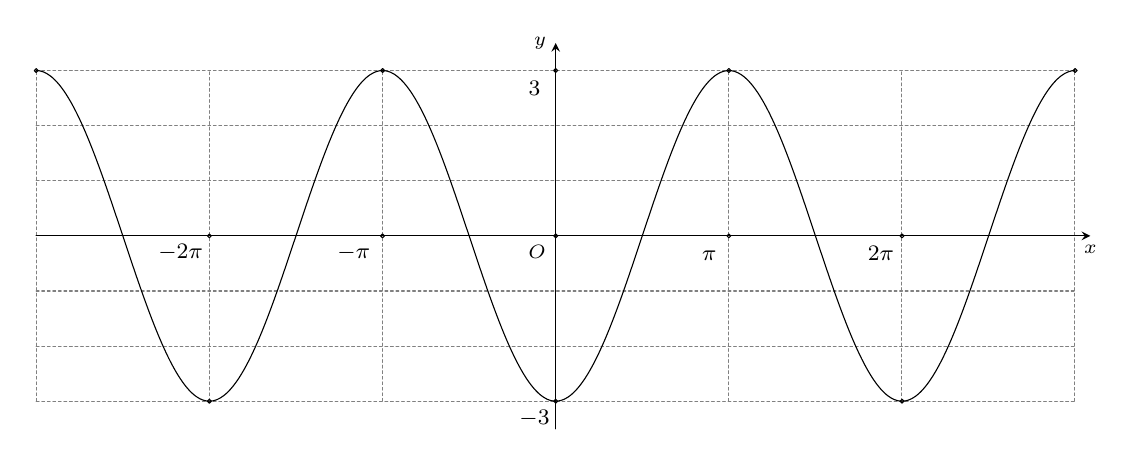
\begin{tikzpicture}[>=stealth,line join=round,line cap=round,font=\footnotesize,scale=0.7]
			\def\a{3.141592654}
			\draw[color=gray,dash pattern=on 1pt off 1pt,xstep=3.14cm,ystep=1.0cm] (-9.424,-3) grid (9.424,3);
			\draw[->] (-9.424,0) -- (9.7,0)node[below]{\scriptsize $x$};
			\draw[->] (0,-3.5) -- (0,3.5) node[left] {\scriptsize $y$};
			\draw (0,0)node[below left]{\scriptsize $O$};
			\clip (-9.58,-3.5)rectangle(9.58,3.5);
			\draw[samples=300,smooth,domain=-9.424:9.424] plot(\x,{-3*cos(\x*180/pi)});
			\path(-2*\a,0)node[shift={(-150:12pt)}]{$-2\pi$}
			(-\a,0)node[shift={(-150:12pt)}]{$-\pi$}
			(\a,0)node[shift={(-135:10pt)}]{$\pi$}
			(2*\a,0)node[shift={(-140:10pt)}]{$2\pi$}
			(0,3)node[shift={(-140:10pt)}]{$3$}
			(0,-3)node[shift={(-140:10pt)}]{$-3$};
			\foreach \x/\y in{-2*\a/0,-\a/0,\a/0,2*\a/0,-3*\a/3,3*\a/3,-2*\a/-3,2*\a/-3,\a/3,-\a/3,0/3,0/-3,0/0}\draw(\x,\y) circle (1pt);
		\end{tikzpicture}
	\end{center}
	\choice
	{\True $y=-3\cos x$}
	{$y=-2-\cos x$}
	{$y=2+|\cos x|$}
	{$y=\cos x-4$}
	\loigiai{
		\begin{itemize}
			\item $y(0)=-3\Rightarrow $ loại $y=\cos x-4$ và $y=2+|\cos x|$.
			\item $y(\pi)=3\Rightarrow $ loại $y=-2-\cos x$.
		\end{itemize}
	}
\end{ex}

\begin{ex}%[1T1Y4-1]
	Điều kiện xác định của hàm số $y=\cot x$ là
	\choice
	{ $x \ne \dfrac{\pi}{8}+k\dfrac{\pi}{2}$}
	{$x \ne \dfrac{\pi}{2}+k\pi$}
	{\True $x \ne k\pi$}
	{$x \ne \dfrac{\pi}{4}+k\pi$}
	\loigiai{
		Hàm số xác định khi và chỉ khi $\sin x \ne 0 \Leftrightarrow x \ne k\pi$, $k \in \mathbb{Z}$.
	}
\end{ex}

\begin{ex}%[1T1B4-5]
	Cho hàm số $y=\sin^2x-\sin x+2$. Gọi $M,N$ lần lượt là GTLN và GTNN của hàm số đã cho. Khi đó $M+N$ bằng
	\choice
	{$k=-\dfrac{1}{2}$}
	{\True $\dfrac{23}{4}$}
	{$\dfrac{15}{4}$}
	{$6$}
	\loigiai{
		Ta có $y=\sin^2x-\sin x+2=\left(\sin x-\dfrac{1}{2}\right)^2+\dfrac{7}{4}$. \\
		Vì $-1 \leq \sin x \leq 1,\,\forall x \in \mathbb{R}$ nên $-\dfrac{3}{2} \leq \sin x-\dfrac{1}{2} \leq \dfrac{1}{2},\,\forall x \in \mathbb{R}$.\\
		Suy ra $0 \leq \left(\sin x-\dfrac{1}{2}\right)^2 \leq \dfrac{9}{4},\,\forall x \in \mathbb{R}$.\\
		Suy ra $\dfrac{7}{4} \leq \left(\sin x-\dfrac{1}{2}\right)^2+\dfrac{7}{4} \leq 4,\,\forall x \in \mathbb{R}$.\\
		Suy ra $\dfrac{7}{4} \leq y \leq 4,\,\forall x \in \mathbb{R}$.\\
		Vậy $M+N=\dfrac{7}{4}+4=\dfrac{23}{4}$.}
\end{ex}

\begin{ex}%[Tex hóa SGK CD-CT,T12/22, TVN-006]%[1K1Y3-4]
	Trong các hàm số sau đây, hàm số nào là hàm tuần hoàn?
	\choice
	{$y=\tan x+x$}
	{$y=x^2+1$}
	{\True $y=\cot x$}
	{$y=\dfrac{\sin x}{x}$}
	\loigiai{
		Hàm số $y=\cot x$ là hàm số tuần hoàn với chu kỳ $T=\pi$.
	}
\end{ex}

\begin{ex}%[1T1Y1-1]
	Góc $18^\circ$ có số đo bằng rađian là bao nhiêu?
	\choice
	{$\pi$}
	{$\dfrac{\pi}{360}$}
	{\True $\dfrac{\pi}{10}$}
	{$\dfrac{\pi}{18}$}
	\loigiai{
		Ta có $18^\circ=\dfrac{\pi}{10}$ rad.
	}
\end{ex}

\begin{ex}%[Tex hóa SGK CD-CT,T12/22, TVN-006]%[1K1Y1-4]
	Biểu diễn các góc lượng giác $\alpha=-\dfrac{5\pi}{6}$, $\beta=\dfrac{\pi}{3}$, $\gamma=\dfrac{25\pi}{3}$, $\delta=\dfrac{17\pi}{6}$ trên đường tròn lượng giác. Các góc nào có điểm biểu diễn trùng nhau?
	\choice
	{\True $\beta$ và $\gamma$}
	{$\alpha$, $\beta$, $\gamma$}
	{$\beta$, $\gamma$, $\delta$}
	{$\alpha$ và $\beta$}
	\loigiai{
		Ta có $\beta+8\pi=\dfrac{\pi}{3}+8\pi=\dfrac{25\pi}{3}=\gamma$.\\
		Do đó, $\beta$ và $\gamma$ có điểm biểu diễn trùng nhau trên đường tròn lượng giác.
	}
\end{ex}

\begin{ex}%[1C1B1-2]
	Cho góc lượng giác $(Ou,Ov)$ có số đo là $\dfrac{3\pi}{4}$, góc lượng giác $(Ou,Ow)$ có số đo là $\dfrac{5\pi}{4}$. Số đo của góc lượng giác $(Ov,Ow)$ là
	\choice
	{\True $(Ov,Ow)=\dfrac{\pi}{2}+k2\pi\ (k\in \mathbb{Z})$}
	{$(Ov,Ow)=2\pi+k2\pi\ (k\in \mathbb{Z})$}
	{$(Ov,Ow)=-\dfrac{\pi}{2}+k2\pi\ (k\in \mathbb{Z})$}
	{$(Ov,Ow)=-\dfrac{\pi}{6}+k2\pi\ (k\in \mathbb{Z})$}
	\loigiai{
		Theo hệ thức Chasles, ta có
		\begin{eqnarray*}
			(Ov,Ow)&=&(Ou,Ow)-(Ou,Ov)+k2\pi\\
			&=&\dfrac{5\pi}{4}-\dfrac{3\pi}{4}+k2\pi\\
			&=&\dfrac{\pi}{2}+k2\pi\ (k\in \mathbb{Z}).
		\end{eqnarray*}
	}
\end{ex}

\begin{ex}%[1C1B1-2]
	Cho góc lượng giác gốc $O$ có tia đầu $Ou$, tia cuối $Ov$ và có số đo $45^\circ$. Cho góc lượng giác $(O'u',O'v')$ có tia đầu $O'u'\equiv Ou$, tia cuối $O'v'\equiv Ov$. Công thức biểu thị số đo góc lượng giác $(O'u',O'v')$ là
	\choice
	{$(O'u',Ov')=-45^\circ+k360^\circ\ (k\in \mathbb{Z})$}
	{\True $(O'u',Ov')=45^\circ+k360^\circ\ (k\in \mathbb{Z})$}
	{$(O'u',Ov')=135^\circ+k360^\circ\ (k\in \mathbb{Z})$}
	{$(O'u',Ov')=-135^\circ+k360^\circ\ (k\in \mathbb{Z})$}
	\loigiai{
		Ta có $(O'u',Ov')=(Ou,Ov)+k360^\circ=45^\circ+k360^\circ\ (k\in \mathbb{Z})$.
	}
\end{ex}

\begin{ex}%[1T1B4-5]
	Hàm số $y=3-5\sin x$ có giá trị lớn nhất bằng
	\choice
	{$6$}
	{$2$}
	{\True $8$}
	{$4$}
	\loigiai{
		Ta có
		$$-1\le \sin x\le 1 \Leftrightarrow 5\ge-5\sin x\ge-5\Leftrightarrow  8\ge 3-5\sin x\ge -2\Rightarrow -2\le y\le 8.$$
		Suy ra giá trị lớn nhất của hàm số là $8$, đạt được khi $x=\dfrac{\pi}{2}+k2\pi,k\in\mathbb{Z}$.
	}
\end{ex}

\begin{ex}%[1T1B2-4]
	Rút gọn biểu thức $M=\sin(\pi-a)+\tan\left(\dfrac{\pi}{2}-a\right)+\sin(-a)+\cot(\pi+a)$ được
	\choice
	{$M=2\cos a$}
	{$M=2\tan a$}
	{\True $M=2\cot a$}
	{$M=0$}
	\loigiai{
		Ta có $M=\sin a+\cot a-\sin a+\cot a=2\cot a$.
	}
\end{ex}

\begin{ex}%[1T1Y4-6]
	Đồ thị hàm số $y=\cos x$ đi qua điểm nào sau đây?
	\choice
	{$P(-1;\pi)$}
	{$M(\pi;1)$}
	{$Q(3\pi; 1)$}
	{\True $N(0;1)$}
	\loigiai{
		Điểm $N(0;1)$ thuộc đồ thị hàm số.
	}
\end{ex}

\begin{ex}%[1T1B4-1]
	Tập xác định của hàm số $y=2017\tan^{2018} \left( 2x+\dfrac{\pi}{3}\right)$ là
	\choice
	{\True $\mathscr{D}=\mathbb{R}\setminus\left\lbrace\dfrac{\pi}{12}+k\dfrac{\pi}{2}, k\in\mathbb{Z} \right\rbrace $}
	{$\mathscr{D}=\mathbb{R}\setminus\left\lbrace\dfrac{\pi}{2}+k\dfrac{\pi}{2}, k\in\mathbb{Z} \right\rbrace $}
	{$\mathscr{D}=\mathbb{R}\setminus\left\lbrace\dfrac{\pi}{2}+k\dfrac{\pi}{2}, k\in\mathbb{Z} \right\rbrace $}
	{$\mathscr{D}=\mathbb{R}\setminus\left\lbrace\dfrac{\pi}{2}+k\dfrac{\pi}{2}, k\in\mathbb{Z} \right\rbrace $}
	\loigiai{
		Hàm số xác định khi $2x+\dfrac{\pi}{3}\ne \dfrac{\pi}{2}+k\pi\Leftrightarrow x\ne\dfrac{\pi}{12}+k\dfrac{\pi}{2}, k\in\mathbb{Z}.$
	}
\end{ex}

% \begin{ex}%[1K1Y1-7]
% 	Tìm khẳng định đúng (với điều kiện các hệ thức đã xác định).
% 	\choice
% 	{$\cos \left(\pi -\alpha \right)=\cos \alpha$}
% 	{\True $\cos \left(-\alpha \right)=\cos \alpha$}
% 	{$\sin \left(\pi -\alpha \right)=-\sin \alpha$}
% 	{$\sin \left(-\alpha \right)=\sin \alpha$}
% 	\loigiai{
% 		Ta có
% 		\begin{itemize}
% 			\item $\sin \left(-\alpha \right)=-\sin \alpha$.
% 			\item $\cos \left(\pi -\alpha \right)=-\cos \alpha$.
% 			\item $\cos \left(-\alpha \right)=\cos \alpha$.
% 			\item $\sin \left(\pi -\alpha \right)=\sin \alpha$.
% 		\end{itemize}
% 	}
% \end{ex}

\TNTF

\begin{ex}%[Pj31--2-Đề KT Theo Bài--TeamTeXHoa--Khổng Xuân Thạnh]%[1D1H5-5] 
	Cho phương trình lượng giác $\sin^2 2x+\cos^2 5x=1$, vậy:
	\choiceTF
	{\True Phương trình đã cho tương đương với phương trình $\dfrac{1-\cos4x}{2}+\dfrac{1+\cos10x}{2}=1$}
	{\True Nghiệm dương nhỏ nhất của phương trình là: $x=\dfrac{\pi}{7}$}
	{Nghiệm âm lớn nhất của phương trình nhỏ hơn $-\dfrac{\pi}{3}$}
	{\True Tổng nghiệm âm lớn nhất và nghiệm dương nhỏ nhất bằng $0$}
	\loigiai{
		\begin{itemchoice}
			\itemch Phương trình tương đương với \[\dfrac{1-\cos4x}{2}+\dfrac{1+\cos10x}{2}=1.\]
			\itemch 	Phương trình tương đương với \[\dfrac{1-\cos4x}{2}+\dfrac{1+\cos10x}{2}=1\Leftrightarrow\cos10x=\cos4x\Leftrightarrow\hoac{&10x=4x+k2\pi\\&10x=-4x+k2\pi}\Leftrightarrow\hoac{&x=\dfrac{k\pi}{3}\\&x=\dfrac{k\pi}{7}.}\]
			Vậy nghiệm dương nhỏ nhất của phương trình là $x=\dfrac{\pi}{7}$.
			\itemch Nghiệm âm lớn nhất của phương trình là $x=-\dfrac{\pi}{7}$.
			\itemch  Tổng nghiệm âm lớn nhất và nghiệm dương nhỏ nhất là $-\dfrac{\pi}{7}+\dfrac{\pi}{7}=0$.
		\end{itemchoice}
	}
\end{ex}

%C16
\begin{ex}%[Pj31--2-Đề KT Theo Bài--TeamTeXHoa--Khổng Xuân Thạnh]%[1D1H5-3]
	Cho phương trình lượng giác $(\sin x+\cos x)^2=2\cos^2 3x$, vậy:
	\choiceTF
	{Phương trình đã cho tương đương với phương trình $1+\sin2x=3+\cos6x$}
	{Nghiệm dương nhỏ nhất của phương trình lớn hơn $\dfrac{\pi}{7}$}
	{\True Nghiệm âm lớn nhất của phương trình là $x=-\dfrac{\pi}{8}$}
	{Tổng nghiệm âm lớn nhất và nghiệm dương nhỏ nhất bằng $0$}
	\loigiai{
		\begin{itemchoice}
			\itemch Ta có \[(\sin x+\cos x)^2=2\cos^2 3x\Leftrightarrow 1+2\sin x\cdot\cos x=1+\cos 6x\Leftrightarrow1+\sin2x=1+\cos6x.\]
			\itemch Ta có
			\begin{eqnarray*}
				&&(\sin x+\cos x)^2=2\cos^2 3x\Leftrightarrow 1+2\sin x\cdot\cos x=1+\cos 6x\\
				&\Leftrightarrow&1+\sin2x=1+\cos6x\Leftrightarrow\cos6x=\sin2x=\cos\left(\dfrac{\pi}{2}-2x\right)\\
				&\Leftrightarrow&\hoac{&6x=\dfrac{\pi}{2}-2x+k2\pi\\&6x=-\dfrac{\pi}{2}+2x+k2\pi}\Leftrightarrow\hoac{&x=\dfrac{\pi}{16}+\dfrac{k\pi}{4}\\&x=-\dfrac{\pi}{8}+\dfrac{k\pi}{2}}\,(k\in \mathbb{Z}).
			\end{eqnarray*}
			Vậy nghiệm dương nhỏ nhất của phương trình lớn hơn $\dfrac{\pi}{16}$.
			\itemch Nghiệm âm lớn nhất của phương trình là $x=-\dfrac{\pi}{8}$
			\itemch  Tổng nghiệm âm lớn nhất và nghiệm dương nhỏ nhất bằng $\dfrac{\pi}{16}-\dfrac{\pi}{8}=-\dfrac{\pi}{16}$.
		\end{itemchoice}
	}
\end{ex}

\begin{ex} %[1D1V3-5]
	Cho $\cos a = \dfrac{1}{3}$, $\cos b = \dfrac{1}{4}$. Khi đó:
	\choiceTF
	{\True $\sin^2 a = \dfrac{8}{9}$}
	{$\sin^2 a > \sin^2 b$}
	{\True $\sin^2 a + \sin^2 b > 1$}
	{$\cos (a+b) \cdot \cos (a-b) = \dfrac{11}{14}$}
	\loigiai{
		\begin{itemize}
			\item Ta có $\sin^2 a = 1 - \cos^2 a = 1 - \dfrac{1}{9} = \dfrac{8}{9}$, $\sin^2 b = 1 - \cos^2 b = 1 - \dfrac{1}{16} = \dfrac{15}{16}$.
			\item So sánh: $\dfrac{8}{9} = \dfrac{128}{144}$ và $\dfrac{15}{16} = \dfrac{135}{144} \Rightarrow \sin^2 a < \sin^2 b$ nên b) Sai.
			\item $\sin^2 a + \sin^2 b = \dfrac{8}{9} + \dfrac{15}{16} = \dfrac{128}{144} + \dfrac{135}{144} = \dfrac{263}{144} > 1$ nên c) Đúng.
			\item
			      \[
				      \cos (a+b) \cdot \cos (a-b) = (\cos a \cos b - \sin a \sin b)(\cos a \cos b + \sin a \sin b) = \cos^2 a \cos^2 b - \sin^2 a \sin^2 b
			      \]
			      \[
				      = \left( \dfrac{1}{3} \right)^2 \cdot \left( \dfrac{1}{4} \right)^2 - \dfrac{8}{9} \cdot \dfrac{15}{16} = \dfrac{1}{9} \cdot \dfrac{1}{16} - \dfrac{8}{9} \cdot \dfrac{15}{16} = \dfrac{1}{144} - \dfrac{120}{144} = -\dfrac{119}{144}.
			      \]
			      Khác $\dfrac{11}{14}$ nên d) Sai.
		\end{itemize}
	}
\end{ex}

\begin{ex} %[1D1V5-5]
	Cho phương trình lượng giác $\sin \left( 3x + \dfrac{\pi}{3} \right) = \cos \left( 2x - \dfrac{\pi}{4} \right)$, vậy:
	\choiceTF
	{\True Phương trình có nghiệm là
		$x = \dfrac{\pi}{12} + \dfrac{k2\pi}{5} \quad \text{hoặc} \quad x = -\dfrac{\pi}{12} + k2\pi, \quad k \in \mathbb{Z}$}
	{Trong khoảng $(-\pi, \pi)$ phương trình có $3$ nghiệm}
	{\True $x = -\dfrac{\pi}{12}$ là một nghiệm của phương trình thuộc khoảng $(-\pi, \pi)$}
	{Tổng các nghiệm trong $(-\pi, \pi)$ bằng $\dfrac{\pi}{4}$}
	\loigiai{
		\begin{itemize}
			\item Giải phương trình:
			      \[
				      \sin \left( 3x + \dfrac{\pi}{3} \right) = \sin \left( \dfrac{3\pi}{4} - 2x \right)
			      \]
			      \[
				      \Leftrightarrow
				      \begin{cases}
					      3x + \dfrac{\pi}{3} = \dfrac{3\pi}{4} - 2x + k2\pi \\
					      \text{hoặc}                                        \\
					      3x + \dfrac{\pi}{3} = \pi - \left( \dfrac{3\pi}{4} - 2x \right) + k2\pi
				      \end{cases}
			      \]
			      Giải ra được:
			      \[
				      x = \dfrac{\pi}{12} + \dfrac{k2\pi}{5} \quad \text{hoặc} \quad x = -\dfrac{\pi}{12} + k2\pi, \quad k \in \mathbb{Z}.
			      \]
			      Vậy a) Đúng.
			\item Với $k = -2, -1, 0, 1, 2$, kiểm tra các nghiệm trong khoảng $(-\pi, \pi)$, được tổng cộng $5$ nghiệm nên b) Sai.
			\item Trong đó có nghiệm $x = -\dfrac{\pi}{12}$ thuộc $(-\pi, \pi)$ nên c) Đúng.
			\item Tổng các nghiệm trong $(-\pi, \pi)$ tính được bằng $\dfrac{\pi}{3}$ nên khác $\dfrac{\pi}{4}$ nên d) Sai.
		\end{itemize}
	}
\end{ex}

\begin{ex} %[1D1V1-4]
	Một đường tròn có bán kính $36\,\mathrm{m}$. Khi đó:
	\choiceTF
	{Cung tròn bán kính $R$ có số đo $\alpha\ (0 \le \alpha \le 2\pi)$, có số đo $a^\circ\ (0 \le a \le 360^\circ)$ và có độ dài là $l$ thì:
		$l = R\alpha = \dfrac{a}{180} \cdot \pi R$}
	{\True Độ dài cung tròn trên đường tròn có số đo $\dfrac{3\pi}{4}$ là $84,8\,\mathrm{m}$}
	{\True Độ dài cung tròn trên đường tròn có số đo $51^\circ$ là $32,04\,\mathrm{m}$}
	{Độ dài cung tròn trên đường tròn có số đo $\dfrac{1}{3}$ là $22\,\mathrm{m}$}
	\loigiai{
		\begin{itemize}
			\item Công thức tính độ dài cung tròn: $l = R\alpha = \dfrac{\pi a}{180} \cdot R$ (với $a^\circ$ là số đo góc).
			\item[a)] $l = 36 \cdot \dfrac{3\pi}{4} = 27\pi \approx 84,8\,\mathrm{m}$ $\rightarrow$ Đúng.
			\item[b)] $l = \dfrac{\pi \cdot 51}{180} \cdot 36 = \dfrac{51\pi}{5} \approx 32,04\,\mathrm{m}$ $\rightarrow$ Đúng.
			\item[c)] $l = 36 \cdot \dfrac{1}{3} = 12\,\mathrm{m}$ $\rightarrow$ Sai (vì kết quả không khớp với $22\,\mathrm{m}$).
		\end{itemize}
	}
\end{ex}

\begin{ex} %[1D1V5-5]
	Cho phương trình lượng giác $\sin^2 2x = \cos^2 \left( 3x - \dfrac{\pi}{8} \right)$, vậy:
	\choiceTF
	{\True Phương trình đã cho tương đương với phương trình $\cos \left( 6x - \dfrac{\pi}{4} \right) = \cos (\pi + 4x)$}
	{\True Trong khoảng $(-\pi, \pi)$ phương trình có $11$ nghiệm}
	{\True $x = \dfrac{37\pi}{40}$ là một nghiệm của phương trình thuộc khoảng $(-\pi, \pi)$}
	{Tổng các nghiệm trong $(-\pi, \pi)$ bằng $\dfrac{7\pi}{9}$}
	\loigiai{
		\begin{itemize}
			\item Phương trình đã cho tương đương với
			      \[
				      \cos \left( 6x - \dfrac{\pi}{4} \right) = \cos (\pi + 4x)
			      \]
			      nên a) Đúng.
			\item Giải phương trình được các nghiệm:
			      \[
				      x = \dfrac{5\pi}{8} + k\pi, \quad x = \dfrac{37\pi}{40} + \dfrac{k\pi}{5}, \quad k \in \mathbb{Z}.
			      \]
			      Đếm được $11$ nghiệm trong $(-\pi, \pi)$ nên b) Đúng.
			\item $x = \dfrac{37\pi}{40}$ là một nghiệm đúng nằm trong $(-\pi, \pi)$ nên c) Đúng.
			\item Tổng các nghiệm đã cho là $\dfrac{7\pi}{8}$ nên khác với $\dfrac{7\pi}{9}$ nên d) Sai.
		\end{itemize}
	}
\end{ex}

\TL

\begin{ex}%[1C1B4-3]
	Giải phương trình:
	\begin{listEX}[3]
		\item $\sin \left(2x-\dfrac{\pi}{3}\right)=-\dfrac{\sqrt{3}}{2}$;
		\item $\sin \left(3x+\dfrac{\pi}{4}\right)=-\dfrac{1}{2}$;
		\item $\cos \left(\dfrac{x}{2}+\dfrac{\pi}{4}\right) =\dfrac{\sqrt{3}}{2}$;
		\item $2\cos 3x+5=3$;
		\item $3\tan x=-\sqrt{3}$;
		\item $\cot x-3=\sqrt{3}\left(1-\cot x\right)$.
	\end{listEX}
	\loigiai{
		\begin{enumerate}[a)]
			\item Ta có
			      \begin{eqnarray*}
				      &&\sin \left(2x-\dfrac{\pi}{3}\right)=-\dfrac{\sqrt{3}}{2}\\
				      &\Leftrightarrow& \sin \left(2x-\dfrac{\pi}{3}\right) =\sin \left(-\dfrac{\pi}{3}\right)\\
				      &\Leftrightarrow& \hoac{
					      &2x-\dfrac{\pi}{3} =-\dfrac{\pi}{3}+k2\pi\\
					      &2x-\dfrac{\pi}{3} = \pi+\dfrac{\pi}{3}+k2\pi}\\
				      &\Leftrightarrow&
				      \hoac{&2x=k2\pi\\&2x=\dfrac{5\pi}{3} +k2\pi}\\
				      &\Leftrightarrow&
				      \hoac{&x=k\pi\\ &x=\dfrac{5\pi}{6}+k\pi} (k\in \mathbb{Z}).
			      \end{eqnarray*}
			\item Ta có
			      \begin{eqnarray*}
				      &&\sin \left(3x+\dfrac{\pi}{4}\right)=-\dfrac{1}{2} \\
				      &\Leftrightarrow& \sin \left(3x+\dfrac{\pi}{4}\right) =\sin \left(-\dfrac{\pi}{6}\right)\\
				      &\Leftrightarrow& \hoac{
					      &3x+\dfrac{\pi}{4} = -\dfrac{\pi}{6}+k2\pi\\
					      &3x+\dfrac{\pi}{4}=\pi -\left(-\dfrac{\pi}{6}\right)+k2\pi} \\
				      &\Leftrightarrow&
				      \hoac{
					      &3x= -\dfrac{5\pi}{12}+k2\pi\\
					      &3x=\dfrac{11\pi}{12}+k2\pi} \\
				      &\Leftrightarrow&
				      \hoac{&x=-\dfrac{5}{36}+\dfrac{k2\pi}{3}\\
					      &x=\dfrac{11\pi}{36}+\dfrac{k2\pi}{3}} (k\in \mathbb{Z}).
			      \end{eqnarray*}
			\item Ta có
			      \begin{eqnarray*}
				      &&\cos \left(\dfrac{x}{2}+\dfrac{\pi}{4}\right) =\dfrac{\sqrt{3}}{2} \\ &\Leftrightarrow& \cos \left(\dfrac{x}{2}+\dfrac{\pi}{4}\right)=\cos \dfrac{\pi}{6}\\
				      &\Leftrightarrow& \hoac{
					      &\dfrac{x}{2}+\dfrac{\pi}{4} = \dfrac{\pi}{6}+k2\pi\\
					      &\dfrac{x}{2}+\dfrac{\pi}{4}= -\dfrac{\pi}{6}+k2\pi}\\
				      &\Leftrightarrow&
				      \hoac{
					      &\dfrac{x}{2}=-\dfrac{\pi}{12}+k2\pi\\
					      &\dfrac{x}{2}=-\dfrac{5\pi}{12}+k2\pi}\\
				      &\Leftrightarrow&
				      \hoac{
					      &x=-\dfrac{\pi}{6}+k4\pi\\
					      &x=-\dfrac{5\pi}{6}+k4\pi} (k\in \mathbb{Z}).
			      \end{eqnarray*}
			\item Ta có $2\cos 3x+5=3 \Leftrightarrow \cos 3x =-1 \Leftrightarrow 3x=\pi+k2\pi \Leftrightarrow x = \dfrac{\pi}{3}+\dfrac{k2\pi}{3}\,\,(k\in \mathbb{Z})$.
			\item Ta có $3\tan x=-\sqrt{3} \Leftrightarrow \tan x =-\dfrac{\sqrt{3}}{3} \Leftrightarrow
				      \tan x=\tan \left(-\dfrac{\pi}{6}\right) \Leftrightarrow x=-\dfrac{\pi}{6}+k\pi\,\, (k\in \mathbb{Z}).$
			\item Ta có
			      \begin{eqnarray*}
				      &&\cot x-3=\sqrt{3}\left(1-\cot x\right)\\
				      &\Leftrightarrow& \cot x-3 =\sqrt{3}-\sqrt{3}\cot x\\
				      &\Leftrightarrow& (1+\sqrt{3})\cot x=\sqrt{3}(1+\sqrt{3})\\
				      &\Leftrightarrow& \cot x=\sqrt{3}\\
				      &\Leftrightarrow& \cot x=\cot \dfrac{\pi}{6}\\
				      &\Leftrightarrow& x=\dfrac{\pi}{6}+k\pi\,\, (k\in \mathbb{Z}).
			      \end{eqnarray*}
		\end{enumerate}
	}
\end{ex}

\begin{ex}%[1C1B4-3]
	Giải phương trình:
	\begin{listEX}[3]
		\item $\sin \left(2x+\dfrac{\pi}{4}\right)=\sin x$;
		\item $\sin 2x=\cos 3x$;
		\item $\cos^2 2x =\cos^2 \left(x+\dfrac{\pi}{6}\right)$.
	\end{listEX}
	\loigiai{
		\begin{enumerate}[a)]
			\item Ta có
			      \[\sin \left(2x+\dfrac{\pi}{4}\right)=\sin x
				      \Leftrightarrow
				      \hoac{&2x+\dfrac{\pi}{4}=x+k2\pi\\&2x+\dfrac{\pi}{4}=\pi-x+k2\pi}
				      \Leftrightarrow \hoac{&x=-\dfrac{\pi}{4}+k2\pi\\&3x=-\dfrac{\pi}{4}+k2\pi} \Leftrightarrow \hoac{&x=-\dfrac{\pi}{4}+k2\pi\\&x=-\dfrac{\pi}{12}+\dfrac{k2\pi}{3}
				      },\, (k\in \mathbb{Z}).\]
			\item Ta có
			      \begin{eqnarray*}
				      \sin 2x=\cos 3x &\Leftrightarrow& \cos 3x =\cos \left(\dfrac{\pi}{2}-2x\right)\\
				      &\Leftrightarrow& \hoac{
					      &3x=\dfrac{\pi}{2}-2x+k2\pi\\
					      &3x=\pi-\left(\dfrac{\pi}{2}-2x\right) +k2\pi}\\
				      &\Leftrightarrow&
				      \hoac{&5x=\dfrac{\pi}{2}+k2\pi\\&x=\dfrac{\pi}{2}+k2\pi}\\
				      &\Leftrightarrow&
				      \hoac{&x=\dfrac{\pi}{12}+\dfrac{k2\pi}{5}\\
					      &x=\dfrac{\pi}{2}+k2\pi}\, (k\in \mathbb{Z}).
			      \end{eqnarray*}
			\item Ta có $\cos^2 2x =\cos^2 \left(x+\dfrac{\pi}{6}\right) \Leftrightarrow
				      \hoac{
					      &\cos 2x=\cos \left(x+\dfrac{\pi}{6}\right) &(1)\\
					      &\cos 2x=-\cos \left(x+\dfrac{\pi}{6}\right). &(2)
				      }$\\
			      +) $(1) \Leftrightarrow \hoac{
					      &2x=x+\dfrac{\pi}{6}+k2\pi\\
					      &2x=-\left(x+\dfrac{\pi}{6}\right)+k2\pi
				      } \Leftrightarrow
				      \hoac{
					      &x=\dfrac{\pi}{6}+k2\pi\\
					      &3x=-\dfrac{\pi}{6}+k2\pi
				      }
				      \Leftrightarrow
				      \hoac{
					      &x=\dfrac{\pi}{6}+k2\pi\\
					      &x=-\dfrac{\pi}{18}+\dfrac{k2\pi}{3}
				      }(k\in \mathbb{Z})$.\\
			      +) $(2) \Leftrightarrow
				      \cos 2x=\cos\left[\pi- \left(x+\dfrac{\pi}{6}\right) \right]
				      \Leftrightarrow
				      \hoac{
					      &2x=\pi- \left(x+\dfrac{\pi}{6}\right)+k2\pi\\
					      &2x=-\left[\pi- \left(x+\dfrac{\pi}{6}\right)\right]+k2\pi
				      } $
			      \[\Leftrightarrow
				      \hoac{
					      &3x=\dfrac{5\pi}{6}+k2\pi\\
					      &x=-\dfrac{5\pi}{6}+k2\pi
				      } \Leftrightarrow
				      \hoac{
					      &x=\dfrac{5\pi}{18}+\dfrac{k2\pi}{3}\\
					      &x=-\dfrac{5\pi}{6}+k2\pi
				      } \,(k\in\mathbb{Z}).\]
		\end{enumerate}
	}
\end{ex}

\begin{ex}Giải các phương trình sau
	\begin{listEX}[2]
		\item $\sin2x-\cos x+2\sin x=1$;
		\item $2\sin ^2 x-5\sin x+3=0$;
		\item $\sqrt{3}\tan^2 x-2\tan x+\sqrt{3}=0$;
		\item $2\cos^2 2x-5\cos 2x+2=0$;
		\item $\sin^2\dfrac{x}{2}+\sin\dfrac{x}{2}-2=0$.
	\end{listEX}
	\loigiai{
		\begin{enumerate}[a)]
			\item $\sin2x-\cos x+2\sin x=1\Leftrightarrow2\sin x\cos x-\cos x+2\sin x-1=0\Leftrightarrow(2\sin x-1)(\cos x+1)=0\\\Leftrightarrow\hoac{&\sin x=\dfrac{1}{2}\\&\cos x=-1}\Leftrightarrow\hoac{&\sin x=\sin\dfrac{\pi}{6}\\&x=(2k+1)\pi}\Leftrightarrow\hoac{&x=\dfrac{\pi}{6}+k2\pi\\&x=\dfrac{5\pi}{6}+k2\pi\\&x=(2k+1)\pi}\,(k\in\mathbb{Z})$;
			\item $2\sin ^2 x-5\sin x+3=0
				      \Leftrightarrow \left(2\sin x-3\right)\left(\sin x-1\right)=0
				      \Leftrightarrow \hoac{&\sin x=\dfrac{3}{2} >1 \text{ (VN)}\\&\sin x=1}
				      \Leftrightarrow x=\dfrac{\pi}{2}+k2\pi,\, (k\in\mathbb{Z})$
			\item $\sqrt{3}\tan^2 x-2\tan x+\sqrt{3}=0\Leftrightarrow \sqrt{3}\left(\tan x - \dfrac{1}{\sqrt{3}}\right)^2 + \dfrac{2}{\sqrt{3}}=0$ (VN);
			\item $2\cos^2 2x-5\cos 2x+2=0
				      \Leftrightarrow\hoac{&\cos2x=2>1 \text{ (VN)}\\&\cos2x=\dfrac{1}{2}}
				      \Leftrightarrow\cos2x=\cos\dfrac{\pi}{3}
				      \Leftrightarrow 2x=\pm\dfrac{\pi}{3}+k2\pi
				      \Leftrightarrow x=\pm\dfrac{\pi}{6}+k\pi,\, (k\in\mathbb{Z})$;
			\item $\sin^2\dfrac{x}{2}+\sin\dfrac{x}{2}-2=0
				      \Leftrightarrow \hoac{&\sin\dfrac{x}{2}=1\\&\sin\dfrac{x}{2}=-2<-1 \text{ (VN)}}
				      \Leftrightarrow \dfrac{x}{2}=\dfrac{\pi}{2}+k2\pi
				      \Leftrightarrow x=\pi+k4\pi,\, (k\in\mathbb{Z})$.
		\end{enumerate}
	}
\end{ex}
%Câu 1
\begin{ex}
	Tìm tập xác định của các hàm số sau
	\begin{listEX}[3]
		\item $y=\dfrac{1+\cos x}{\sin 2x}$.
		\item $y=\sqrt{\dfrac{1+\cos x}{2+\cos x}}$.
		\item $y=\dfrac{\cos x}{1-\sin x}$.
		\item $y=\dfrac{1}{\tan x}$.
		\item $y=\dfrac{\sqrt{1-\sin x}}{2\cos x-\sqrt{3}}$.
	\end{listEX}
	\loigiai{
		\begin{enumerate}[a)]
			\item $y=\dfrac{1+\cos x}{\sin 2x}$\\
			      Hàm số $y=\dfrac{1+\cos x}{\sin 2x}$ xác định $\Leftrightarrow \sin 2x\ne 0\Leftrightarrow x\ne \dfrac{k\pi }{2},k\in \mathbb{Z}$.\\
			      Vậy $D=\mathbb{R}\setminus \left\{ k\dfrac{\pi }{2},k\in \mathbb{Z} \right\}$.
			\item $y=\sqrt{\dfrac{1+\cos x}{2+\cos x}}$\\
			      Hàm số $y=\sqrt{\dfrac{1+\cos x}{2+\cos x}}$ xác định $\Leftrightarrow \dfrac{1+\cos x}{2+\cos x}\ge 0$\\
			      Ta có: $\heva{& 1+\cos x\ge 0\ ,\ \forall x\in \mathbb{R} \\& 2+\cos x>0\ ,\ \forall x\in \mathbb{R}}\Rightarrow \dfrac{1+\cos x}{2+\cos x}\ge 0\ ,\forall x\in \mathbb{R}$\\
			      Vậy $D=\mathbb{R}$.
			\item $y=\dfrac{\cos x}{1-\sin x}$\\
			      Hàm số $y=\dfrac{\cos x}{1-\sin x}$ xác định $\Leftrightarrow 1-\sin x\ne 0\Leftrightarrow x\ne \dfrac{\pi }{2}+k2\pi $, $k\in \mathbb{Z}$.\\
			      Vậy $D=\mathbb{R}\setminus \left\{ \dfrac{\pi }{2}+k2\pi ,k\in \mathbb{Z} \right\}$.
			\item $y=\dfrac{1}{\tan x}$\\
			      Hàm số $y=\dfrac{1}{\tan x}$ xác định $\Leftrightarrow \heva{& \tan x\ne 0 \\& \cos x\ne 0}\Leftrightarrow \heva{& \sin x\ne 0 \\& \cos x\ne 0}\Leftrightarrow \sin 2x\ne 0\Leftrightarrow x\ne k\dfrac{\pi }{2}$, $k\in \mathbb{Z}$.\\
			      Vậy $D=\mathbb{R}\setminus \left\{ k\dfrac{\pi }{2},k\in \mathbb{Z} \right\}$.
			\item $y=\dfrac{\sqrt{1-\sin x}}{2\cos x-\sqrt{3}}$\\
			      Hàm số $y=\dfrac{\sqrt{1-\sin x}}{2\cos x-\sqrt{3}}$ xác định $\Leftrightarrow \heva{& 1-\sin x\ge 0 \\& 2\cos x-\sqrt{3}\ne 0}$.\\
			      Ta có: $1-\sin x\ge 0\Leftrightarrow \sin x\le 1$, điều này đúng với mọi $x\in \mathbb{R}$.\\
			      $2\cos x-\sqrt{3}\ne 0\Leftrightarrow \cos x\ne \dfrac{\sqrt{3}}{2}\Leftrightarrow x\ne \pm \dfrac{\pi }{6}+k2\pi $, $k\in \mathbb{Z}$.\\
			      Vậy $D=\mathbb{R}\setminus \left\{ \pm \dfrac{\pi }{6}+k2\pi ,k\in \mathbb{Z} \right\}$.
		\end{enumerate}
	}
\end{ex}
%Câu 2
\begin{ex}
	Tìm tập giá trị của các hàm số sau:
	\begin{listEX}[2]
		\item $y=2\sin \left(x+\dfrac{\pi }{4}\right)+3$;
		\item $y=\sqrt{2+\cos x}-5$.
		\item $y=2\cos \left(x-\dfrac{\pi }{4}\right)-7$;
		\item $y=3-\sqrt{2+\sin x}$
	\end{listEX}
	\loigiai{
		\begin{enumerate}
			\item Tập xác định của hàm số là $D=\mathbb{R}$.\\
			      Ta có $-1\le \sin \left(x+\dfrac{\pi }{4}\right)\le 1,\forall x\in \mathbb{R}$\\
			      $\Leftrightarrow -2\le 2\sin \left(x+\dfrac{\pi }{4}\right)\le 2,\forall x\in \mathbb{R}$\\
			      $\Leftrightarrow 1\le 2\sin \left(x+\dfrac{\pi }{4}\right)+3\le 5,\forall x\in \mathbb{R}$\\
			      hay $1\le y\le 5,\forall x\in \mathbb{R}$.\\
			      Vậy tập giá trị của hàm số là $T=\left[1;5\right]$.
			\item Vì $\cos x\ge -1\Leftrightarrow 2+\cos x\ge 1>0,\forall x\in \mathbb{R}$ nên tập xác định của hàm số là $D=\mathbb{R}$.\\
			      Ta có:\\
			      $-1\le \cos x\le 1,\forall x\in \mathbb{R}\Leftrightarrow 1\le 2+\cos x\le 3,\forall x\in \mathbb{R}$ $\Leftrightarrow 1\le \sqrt{2+\cos x}\le \sqrt{3}\,,\forall x\in \mathbb{R}$ $\Leftrightarrow -4\le \sqrt{2+\cos x}\,-5\le \sqrt{3}-5\,,\forall x\in \mathbb{R}$ hay $-4\le y\le \sqrt{3}-5\,,\forall x\in \mathbb{R}$.\\
			      Vậy tập giá trị của hàm số là $T=\left[-4;\sqrt{3}-5\right]$.
			\item Tập xác định của hàm số là $D=\mathbb{R}$.\\
			      Ta có $-1\le \cos \left(x-\dfrac{\pi }{4}\right)\le 1,\forall x\in \mathbb{R}$\\
			      $\Leftrightarrow -2\le 2\cos \left(x-\dfrac{\pi }{4}\right)\le 2,\forall x\in \mathbb{R}$\\
			      $\Leftrightarrow -9\le 2\cos \left(x-\dfrac{\pi }{4}\right)-7\le -5,\forall x\in \mathbb{R}$\\
			      hay $-9\le y\le -5,\forall x\in \mathbb{R}$.\\
			      Vậy tập giá trị của hàm số là $T=\left[-9;-5\right]$.
			\item Vì $2+\sin x\ge 1>0,\forall x\in \mathbb{R}$ nên tập xác định của hàm số là $D=\mathbb{R}$.\\
			      Ta có: $-1\le \sin x\le 1,\forall x\in \mathbb{R}$\\
			      $\Leftrightarrow 1\le 2+\sin x\le 3,\forall x\in \mathbb{R}$\\
			      $\Leftrightarrow 1\le \sqrt{2+\sin x}\le \sqrt{3}\,,\forall x\in \mathbb{R}$\\
			      $\Leftrightarrow -1\ge -\sqrt{2+\sin x}\ge -\sqrt{3}\,,\forall x\in \mathbb{R}$\\
			      $\Leftrightarrow 2\ge 3-\sqrt{2+\sin x}\ge 3-\sqrt{3}\,,\forall x\in \mathbb{R}$\\
			      hay $3-\sqrt{3}\le y\le 2\,,\forall x\in \mathbb{R}$.\\
			      Vậy tập giá trị của hàm số là $T=\left[3-\sqrt{3};2\right]$.
		\end{enumerate}
	}
\end{ex}

\begin{ex}%[1D1G1-5]
	Tìm giá trị lớn nhất và giá trị nhỏ nhất của hàm số  $y=2(\sin x+\cos x)+\sin 2 x+3$.
	\loigiai
	{Tập xác định $\mathscr{D}=\mathbb{R}$.\\
		Đặt $t=\sin x+ \cos x=\sqrt{2}\sin \left(x+\dfrac{\pi}{4}\right)$, $t\in \left[-\sqrt{2};\sqrt{2}\right]$.\\
		Ta có $t^2=\left(\sin x+ \cos x\right)^2=1+2\sin x\cos x=1+\sin 2x\Rightarrow \sin 2x =t^2-1$.\\
		Hàm số trở thành $y=g(t)=t^2+2t+2$. \\
		Bảng biến thiên của hàm số $y=g(t)$ trên đoạn $ \left[-\sqrt{2};\sqrt{2}\right]$
		\begin{center}
			
\begin{tikzpicture}
				\tkzTabInit[lgt=1,espcl=3,deltacl=1]%nocadre,
				{$t$/1, $g(t)$ /2}
				{$-\sqrt{2}$ , $-1$ ,  $\sqrt{2}$}
				\tkzTabVar {+/$4-2\sqrt{2}$,-/$1$ ,+/ $4+2\sqrt{2}$}
			\end{tikzpicture}
		\end{center}
		Vậy $\max\limits_{x \in \mathbb{R}} y=4+2\sqrt{2}$ và $\min\limits_{x \in \mathbb{R}} y=1$.
	}
\end{ex}

\begin{ex}%[1D1K1-5]
	Tìm giá trị lớn nhất và giá trị nhỏ nhất của hàm số $y=\sqrt{3} \sin x-\cos x+5$.
	\loigiai
	{
		Tập xác định $\mathscr{D}=\mathbb{R}$.\\
		Biến đổi $y=\sqrt{3} \sin x-\cos x+5=2\left(\dfrac{\sqrt{3}}{2}\cdot\sin x-\dfrac{1}{2}\cdot\cos x\right)+5=2\sin\left(x-\dfrac{\pi}{6}\right)+5$.\\
		Với mọi $x\in \mathbb{R}$ ta có
		\allowdisplaybreaks
		\begin{eqnarray*}
			& & -1\leq \sin\left(x-\dfrac{\pi}{6}\right)\leq 1\\
			&\Leftrightarrow& -2\leq 2\sin\left(x-\dfrac{\pi}{6}\right)\leq 2\\
			&\Leftrightarrow&3\leq  2\sin\left(x-\dfrac{\pi}{6}\right)+5\leq 7.
		\end{eqnarray*}
		Vậy $\max\limits_{x \in \mathbb{R}} y=7$ khi $x=\dfrac{2\pi}{3}$ và $\min\limits_{x \in \mathbb{R}} y=3$ khi $x=-\dfrac{\pi}{3}$.
	}
\end{ex}

\begin{ex}%[1D1V4-7]%[BG K11, Nhật Thiện][Chân trời sáng tạo - Mức độ 3]
	\immini[thm]{Trong Địa lí, phép chiếu hình trụ được sử dụng để vẽ một bản đồ phẳng như trong hình bên. Trên bản đồ phẳng lấy đường xích đạo làm trục hoành và kinh tuyến $0^{\circ}$ làm trục tung. Khi đó tung độ của một điểm có vĩ độ $\varphi^{\circ}$ $(-90<\varphi<90)$ được cho bởi hàm số $y=20 \tan \left(\dfrac{\pi}{180} \varphi\right)$ (cm).
		Sử dụng đồ thị hàm số tan, hãy cho biết những điểm ở vĩ độ nào nằm cách xích đạo không quá $20$ (cm) trên bản đồ? (Theo https://geologyscience.com/geology/types-of-maps/).}
	{
		\includegraphics[scale=0.45]{hinhve/CTST/CTST-1_4_1}
	}
	\loigiai{
	\immini{Vì điểm nằm cách xích đạo không quá $20$ (cm) trên bản đồ nên ta có $-20 \leq y \leq 20$.\\
	Khi đó $-20 \leq 20 \tan \left(\dfrac{\pi}{180} \varphi\right) \leq 20$ hay $-1 \leq \tan \left(\dfrac{\pi}{180} \varphi\right) \leq 1$.\\
	Ta có $-90<\varphi<90$ khi và chi khi $-\dfrac{\pi}{2}<\dfrac{\pi}{180} \varphi<\dfrac{\pi}{2}$.\\
	Xét đồ thị hàm số $y=\tan x$ trên khoảng $\left(-\dfrac{\pi}{2} ; \dfrac{\pi}{2}\right)$ (Hình vẽ bên).\\
	Ta thấy $-1 \leq \tan \left(\dfrac{\pi}{180} \varphi\right) \leq 1$ khi và chi khi $-\dfrac{\pi}{4} \leq \dfrac{\pi}{180} \varphi \leq \dfrac{\pi}{4}$ hay $-45 \leq \varphi \leq 45$.\\
	Vậy trên bản đồ, các điểm cách xích đạo không quá $20$ (cm)
	nằm ở vĩ độ từ $-45^{\circ}$ đến $45^{\circ}$.}
	{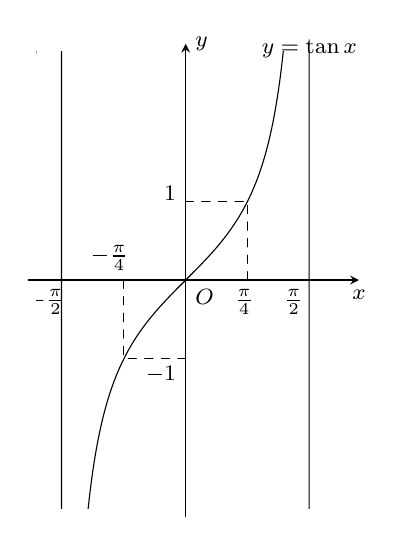
\begin{tikzpicture}[scale=1,>=stealth, font=\footnotesize, line join=round, line cap=round]
		\def\xmin{-2} \def\xmax{2.2} \def\ymin{-3} \def\ymax{3}
		\draw[->] (\xmin,0)--(\xmax,0) node [below]{$x$};
		\draw[->] (0,\ymin)--(0,\ymax) node [right]{$y$};
		\node at (0,0) [below right]{$O$};
		\node at (0.3*pi-0.1,2.7) [above right]{$y=\tan x$};
		\clip (\xmin+0.1,\ymin+0.1) rectangle (\xmax-0.5,\ymax-0.1);
		\draw[smooth,samples=400,domain=\xmin:\xmax] plot(\x,{tan(\x r)});
		\node at (0,1.1) [left]{$1$};
		\node at (0,-1.2) [left]{$-1$};
		\node at (-0.18*pi-0.4,0) [above]{$-\frac{\pi}{4}$};
		\node at (0.3*pi-0.2,0) [below]{$\frac{\pi}{4}$};
		\node at (-2*pi-0.2,0) [above]{$-2\pi$};
		\node at (-1.5*pi-0.4,0) [below]{$-\frac{3\pi}{2}$};
		\node at (-pi-0.2,0) [above]{$-\pi$};
		\node at (-0.5*pi-0.2,0) [below]{$-\frac{\pi}{2}$};
		\node at (0.5*pi-0.2,0) [below]{$\frac{\pi}{2}$};
		\node at (1.5*pi-0.3,0) [below]{$\frac{3\pi}{2}$};
		\node at (2*pi+0.2,0) [below]{$2\pi$};
		\draw[dashed] (0.25*pi,0)--(0.25*pi,1)--(0,1);
		\draw[dashed] (-0.25*pi,0)--(-0.25*pi,-1)--(0,-1);
	\end{tikzpicture}}
	}
\end{ex}


\Closesolutionfile{ans}